\documentclass[a4paper,11pt]{article}
\usepackage[utf8]{inputenc}
\usepackage{textcomp}
\usepackage{lmodern}
\usepackage{listings}
\usepackage{graphicx}
\usepackage{listings}
\usepackage{color}
\usepackage{url}
\usepackage{verbatim}
\usepackage[top=3cm,bottom=3cm,left=3cm,right=3cm]{geometry}

\title{Master in Cyber-Security\\
	LINGI2146 --- Mobile and Embedded Computing: \\
	Publishing IoT Sensor Data through a MQTT publish/subscribe infrastructure}

\author{FONTAINE Romain, NYAKI Loïc, TIO NOGUERAS Gérard}

\begin{document}
\maketitle
\newpage
\tableofcontents

\newpage

\section{Introduction}
When using sensors to measure data, such as light, temperature or noise, it is common to use IoT devices: a small battery-powered piece of hardware, equipped with one or several sensors, that can communicate data wirelessly.\\

The way to propagate information is by communicating with neighbouring devices, which will forward the information towards a specific node of the network, called the \textit{root node}. To be able to communicate in this manner, each device must form a relationship with the other nodes and form what is called a Wireless Mesh Network (WMN).\\

Another part of this system is the MQTT infrastructure. MQTT (Message Queuing Telemetry Transport) is a publish/subscribe messaging protocol that allows publishers to publish data to a MQTT broker, while clients can subscribe to that same broker, to receive specific information from the publishers.\\

The first goal of this project is to implement a custom routing protocol, similar to RPL,  that will allow the creation of a network of IoT devices called  Destination Oriented Directed Acyclic Graph, or DODAG for short. Information should be able to travel from any node of the network, to the root node, which acts as a gateway towards the outside world. \\

The second goal is to create an MQTT infrastructure, that allow clients to subscribe to a MQTT broker, and publishers to publish data to the broker.\\

The third and last goal is then to create a \textit{Gateway agent} that will serve as an interface between the IoT network and the MQTT infrastructure, in such a way that the IoT devices should be able to become MQTT publishers, and any client from outside the IoT network should be able to subscribe to the MQTT broker, and be periodically updated with data from the IoT network sensors.

\begin{comment}
First, we need implement a custom routing protocol for sensor networks, similar to RPL, on top of 6LoWPAN which is a special version of IPv6 for low-power devices. Then, we build a messaging infrastructure using MQTT, which is a publish/subscribe messaging protocol. Lastly, we interface the sensor network with the MQTT message infrastructure, by using a border router, whose job will be to translate the message travelling between the sensor network and the MQTT message infrastructure.
\\
Lastly, the sensor data 
\end{comment}
\section{Overview of the System}
The scope of this project covers three separate parts (see figure \ref{fig:architecture1}):
\begin{itemize}
\item{An IoT sensor network, where devices organize themselves, and communicate with each other by using a custom routing protocol similar to RPL.}
\item{A MQTT publish/subscribe infrastructure composed of a MQTT broker and several MQTT client that can either publish data and subscribe to topics to receive data.}
\item{A Rime-MQTT Gateway which interfaces the sensor network with the MQTT infrastructure in order for the IoT network and MQTT infrastructure to talk to each other in a transparent manner.}
\end{itemize}

\begin{figure}
  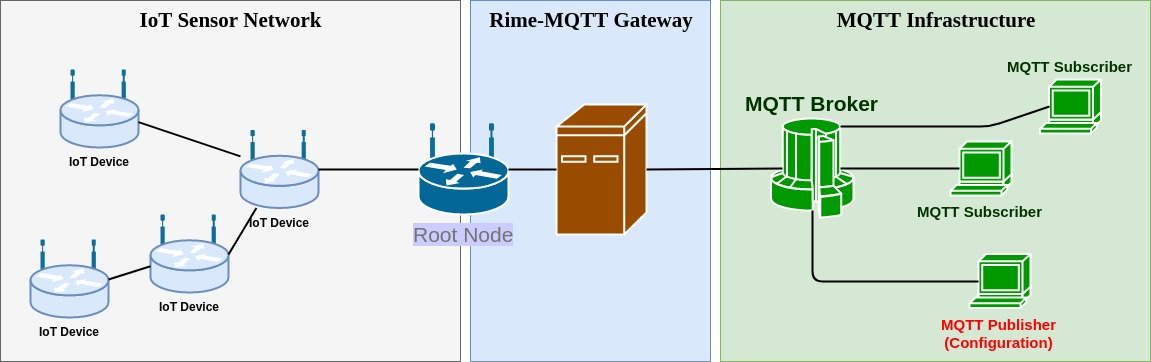
\includegraphics[width=\linewidth]{img/architecture-2.jpg}
  \caption{An overview of the system.}
  \label{fig:architecture1}
\end{figure}
\section{DODAG and Routing Protocol}
One of the objectives of this project is the implementation of a routing protocol, similar to RPL (Routing Protocol for Low-Power and Lossy Networks). A routing protocol is needed in order create a Destination Oriented Directed Acyclic Graph (DODAG), and have the information propagate properly from any individual node to the root node of the network.\\

Any given node that isn't part of the network should have the posibility to become one, and start publishing information. Any node of the network should also be able to disappear without compromising the integrity of the network as long as the node is not a critical junction of two parts of the network graph.

\subsection{Joining a graph}
When an IoT device is started, it needs to find a network to join. It will therefore use a \textit{Discovery message} to broadcast its existence, ask around for some information about the DODAG, and wait for the response. This \textit{Discovery message} will be send periodically based on a timer.\\

When a node that is already a member of the DODAG receives this broadcasted message, it replies with a unicast \textit{Parent Message}, advertising itself as a possible parent. When the node that is trying to join the network receives a \textit{Parent Message}, it saves the address of the parent and sends a unicast \textit{Parent-ACK message} to the parent, to confirm their child-parent relationship. The parent then adds the child to the list of its children.

\subsection{Leaving a graph TODO}
When a node disappears from the DODAG...

\subsection{Sending Sensor Data}
Periodically, each node uses a \textit{ROOT message} to send data to the root node of the DODAG, , which will then forward it to the Gateway, where it will be translated into a MQTT message that will be sent to the MQTT broker. Once it reaches the MQTT broker, the message is forwarded to all the MQTT client that have subscribed to the specific topic relative to that message.

\subsection{Summary of Routing Message Types}
\subsubsection{Discovery Message}
When a node has doesn't belong to the network, it will try sending a broadcast request for potential parent nodes to manifest themselves. This is called a \textit{Discovery message}.

\subsubsection{Parent Message}
A \textit{Parent Message} is sent by a member of the network after receiving a Discovery message. This message advertises the parent's address as well as rank within the network.

\subsubsection{ACK-Parent}
When a node which isn't part of the network receives a \textit{Parent message}, it can decide to set the sender of the \textit{Parent message} as its own parent.it then sends a unicast \textit{ACK-Parent message} to the parent, to inform it that it has a new child. After sending this \textit{ACK-Parent message}, the child node officially becomes part of the network.
\subsubsection{ACK-Info Message}

\subsubsection{Information Message}
Periodically, each node sends takes information from it's sensors and sends it to its parent. To do this, an \textit{Information message} is used.

\subsubsection{Root Message}



\section{MQTT infrastructure}
MQTT stands for Message Queuing Telemetry Transport, and is a publish/subscribe protocol. It requires a MQTT broker as well as MQTT clients that can publish information to the broker, as topics, or subscribe to the broker for a specific topic, in order to be given the required information through time.

\subsection{MQTT Broker}
The broker is the central element of MQTT. It is where each MQTT client either subscribe to a topic, or publishes information under a specific topic. In this instance, we used Mosquitto, an open-source MQTT broker.\\

In our case, the MQTT broker will be running on a regular laptop.


\subsection{MQTT Publishers}
In this project, we have two distinct MQTT publishers. The first MQTT publisher is the \textbf{Rime-MQTT Gateway}, which publishes topics on behalf of the sensor network nodes.\\

The second publisher is the \textbf{MQTT client} used for configuring the sensor network. We use this MQTT configuration client to send configuration commands to the sensor network, in place of using a direct command line interface on the Gateway machine.

\subsection{MQTT Subscribers}
The MQTT broker allows for clients to both publish data, or subscribe in order to be kept updated on data. In this project, we have two different MQTT subscribers : regular MQTT clients, and the Rime-MQTT Gateway.

\subsection{Regular MQTT clients}
For demonstration purpose, one or several clients will run on our machine, and subscribe to specific topics, to receive information from the sensor network. Once subscribed to the appropriate topic, each subscriber will receive periodical information from the network.

\subsection{Rime-MQTT Gateway as a client}
In order to implement the possibility of modifying the IoT network configuration dynamically, we need the Rime-MQTT Gateway to subscribe to a "configuration" topic to the MQTT broker. A specific client will then, when necessary publish configuration commands that will be forwarded to the Gateway.


\section{Rime-MQTT Gateway}
The Rime-MQTT Gateway is a python program, that serves as an interface between the sensor network and the MQTT broker.\\

On one side, it receives data from the root node of the sensor network and translates them into MQTT publish messages that it sends to the MQTT broker. On the other side, it subscribes to the MQTT broker for configurations messages that it then translate into a format that the root of the sensor node understands.\\

\subsection{Prevention of Meaningless Communication}
Most IoT object are powered by battery and are therefore under strict energy requirements. It is of the utmost importance that the battery life be preserved as much as possible. As a consequence, we want to avoid sending data when no one is asking for it.\\

In order to do that, the Gateway subscribes to a MQTT topic that counts the number of people subscribed to the MQTT topics published by the sensor network (\$SYS/broker/subscriptions/count). When the number of subscribers change, the Gateway receives an update.\\

When no one is subscribed, the Gateway sends a message to the network, to tell the nodes that they need to stop sending data, therefore saving their battery life.

The Gateway also subscribes to the  topic, in order to be warned when 

\begin{figure}
  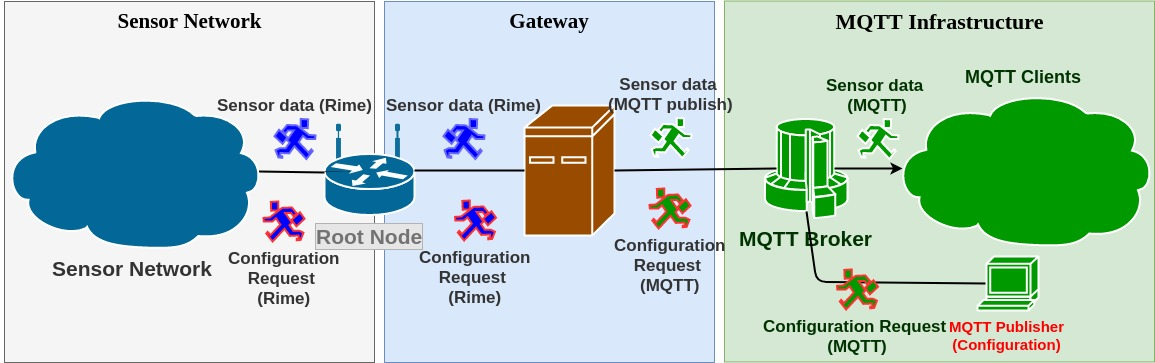
\includegraphics[width=\linewidth]{img/communication-2.jpg}
  \caption{This schema shows how data transits through the Rime-MQTT Gateway.}
  \label{fig:communication1}
\end{figure}

\subsection{Sensor Network Configuration}
One of the requirement of this project is the possibility to dynamically modify the configuration of the sensor network. The proposed method was to by directly interacting with 
\end{document}

